%%%% Figures for ZeeGSFSel Efficiency  %%%%%
\begin{figure}
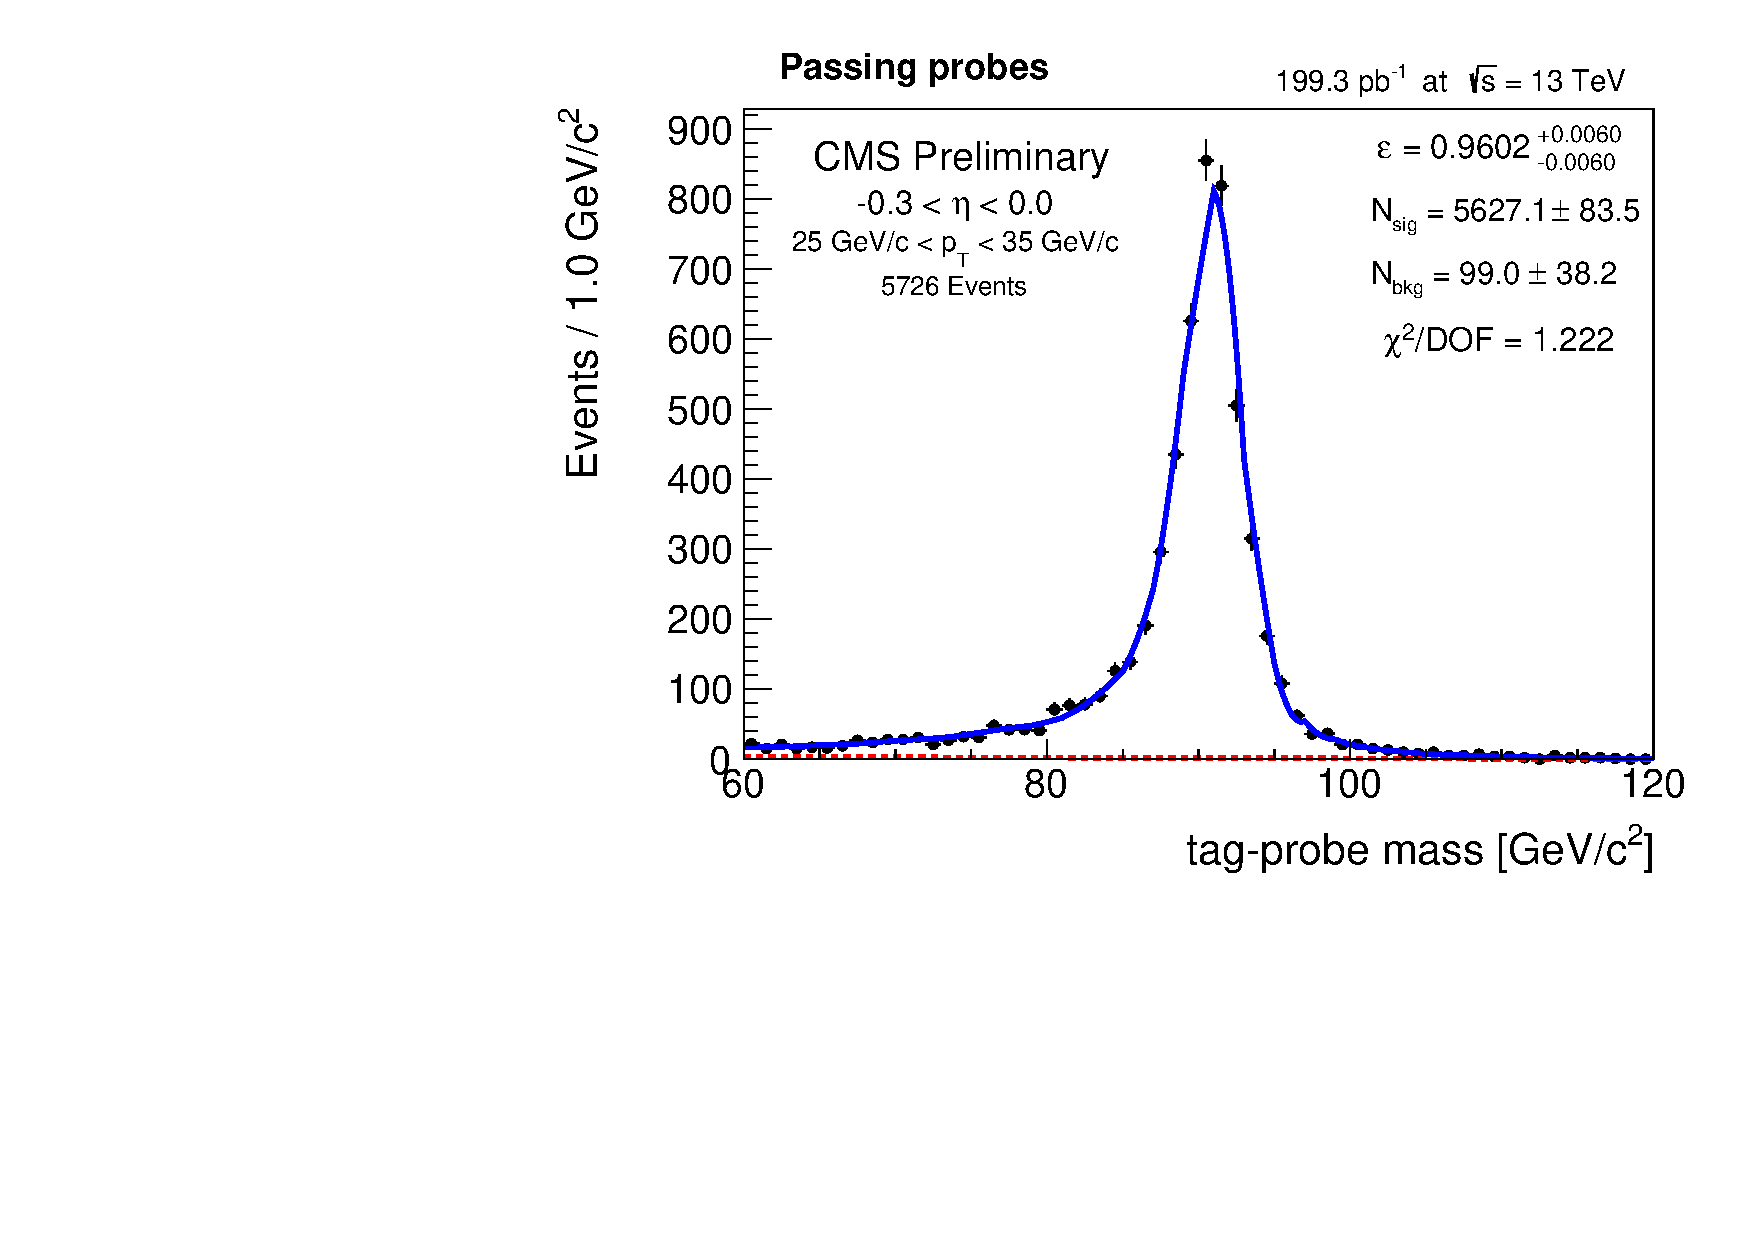
\includegraphics[width=.49\linewidth]{plots/efficiency/examples_musta/passetapt_5.pdf}
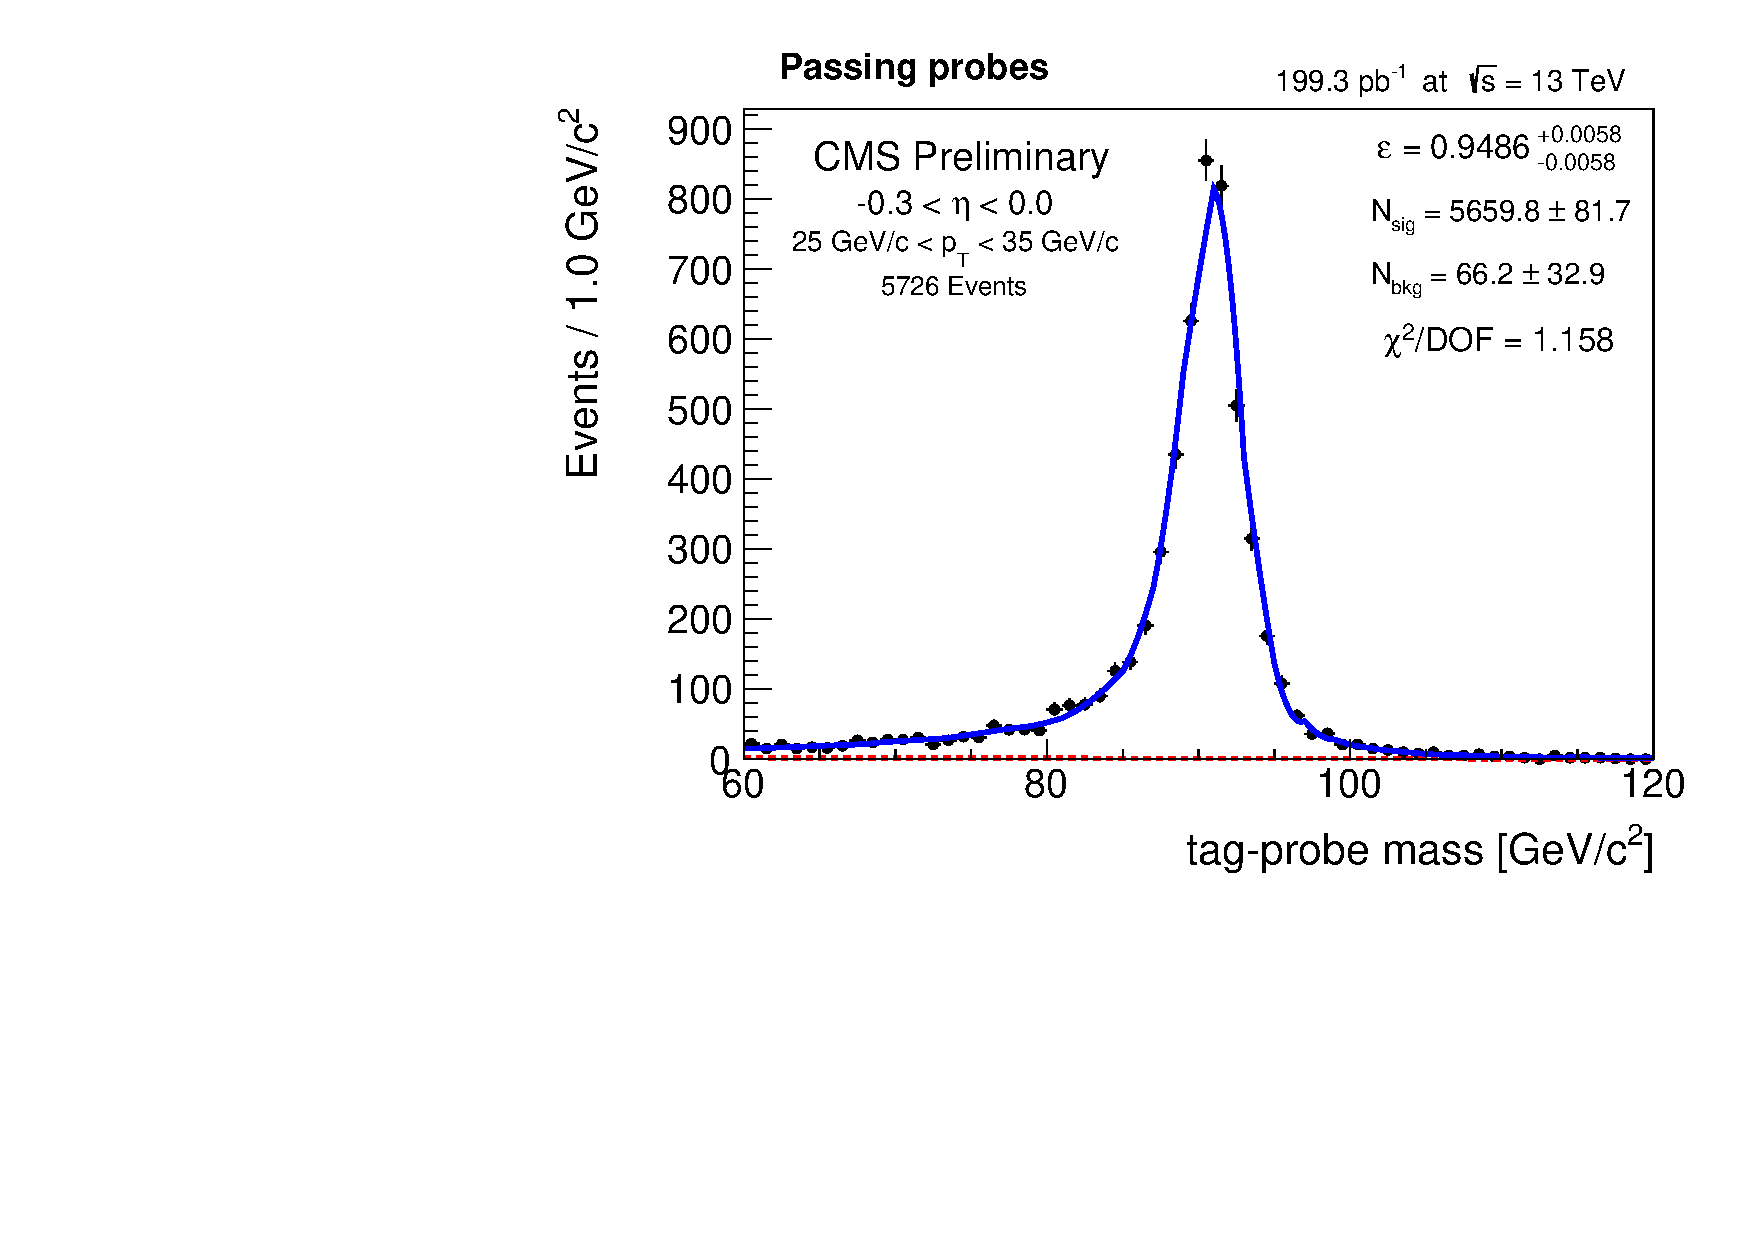
\includegraphics[width=.49\linewidth]{plots/efficiency/examples_plbkg/passetapt_5.pdf}
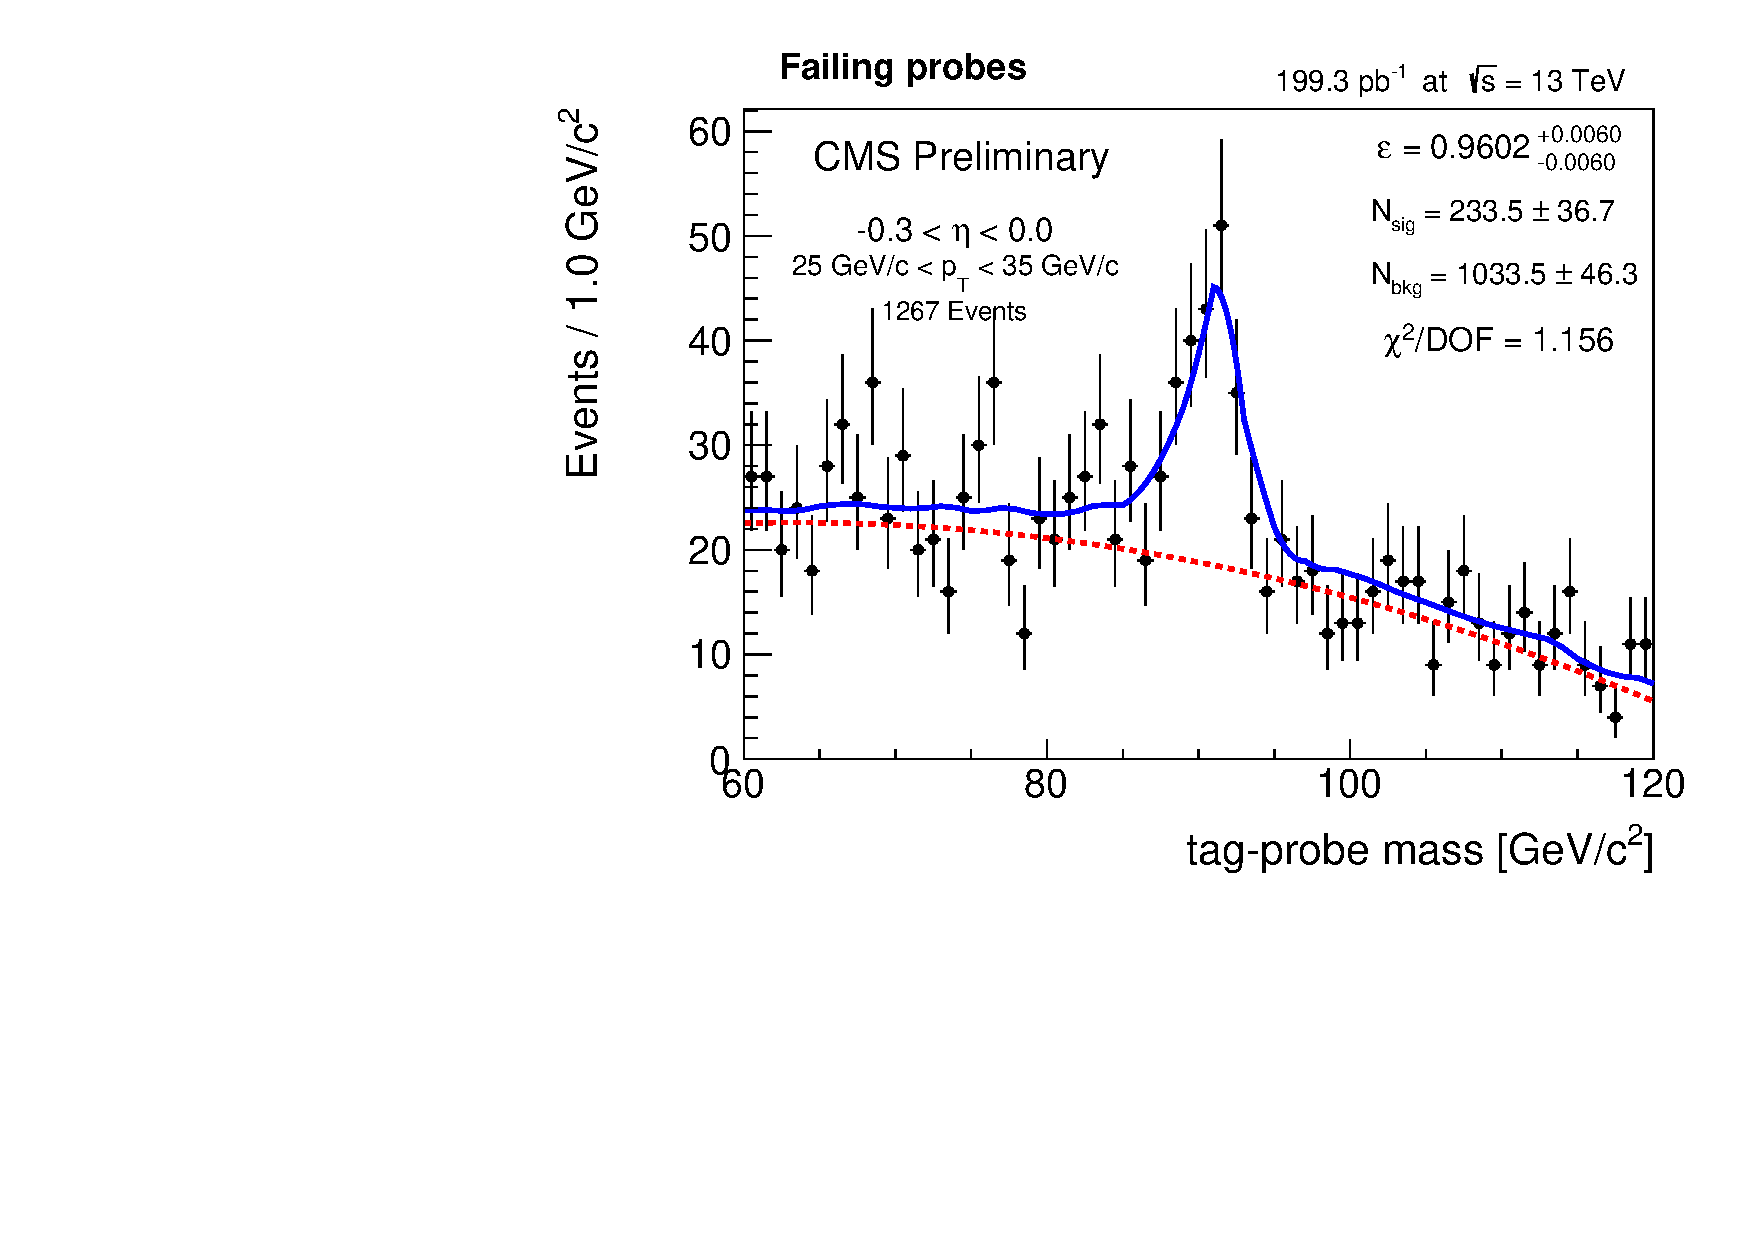
\includegraphics[width=.49\linewidth]{plots/efficiency/examples_musta/failetapt_5.pdf}
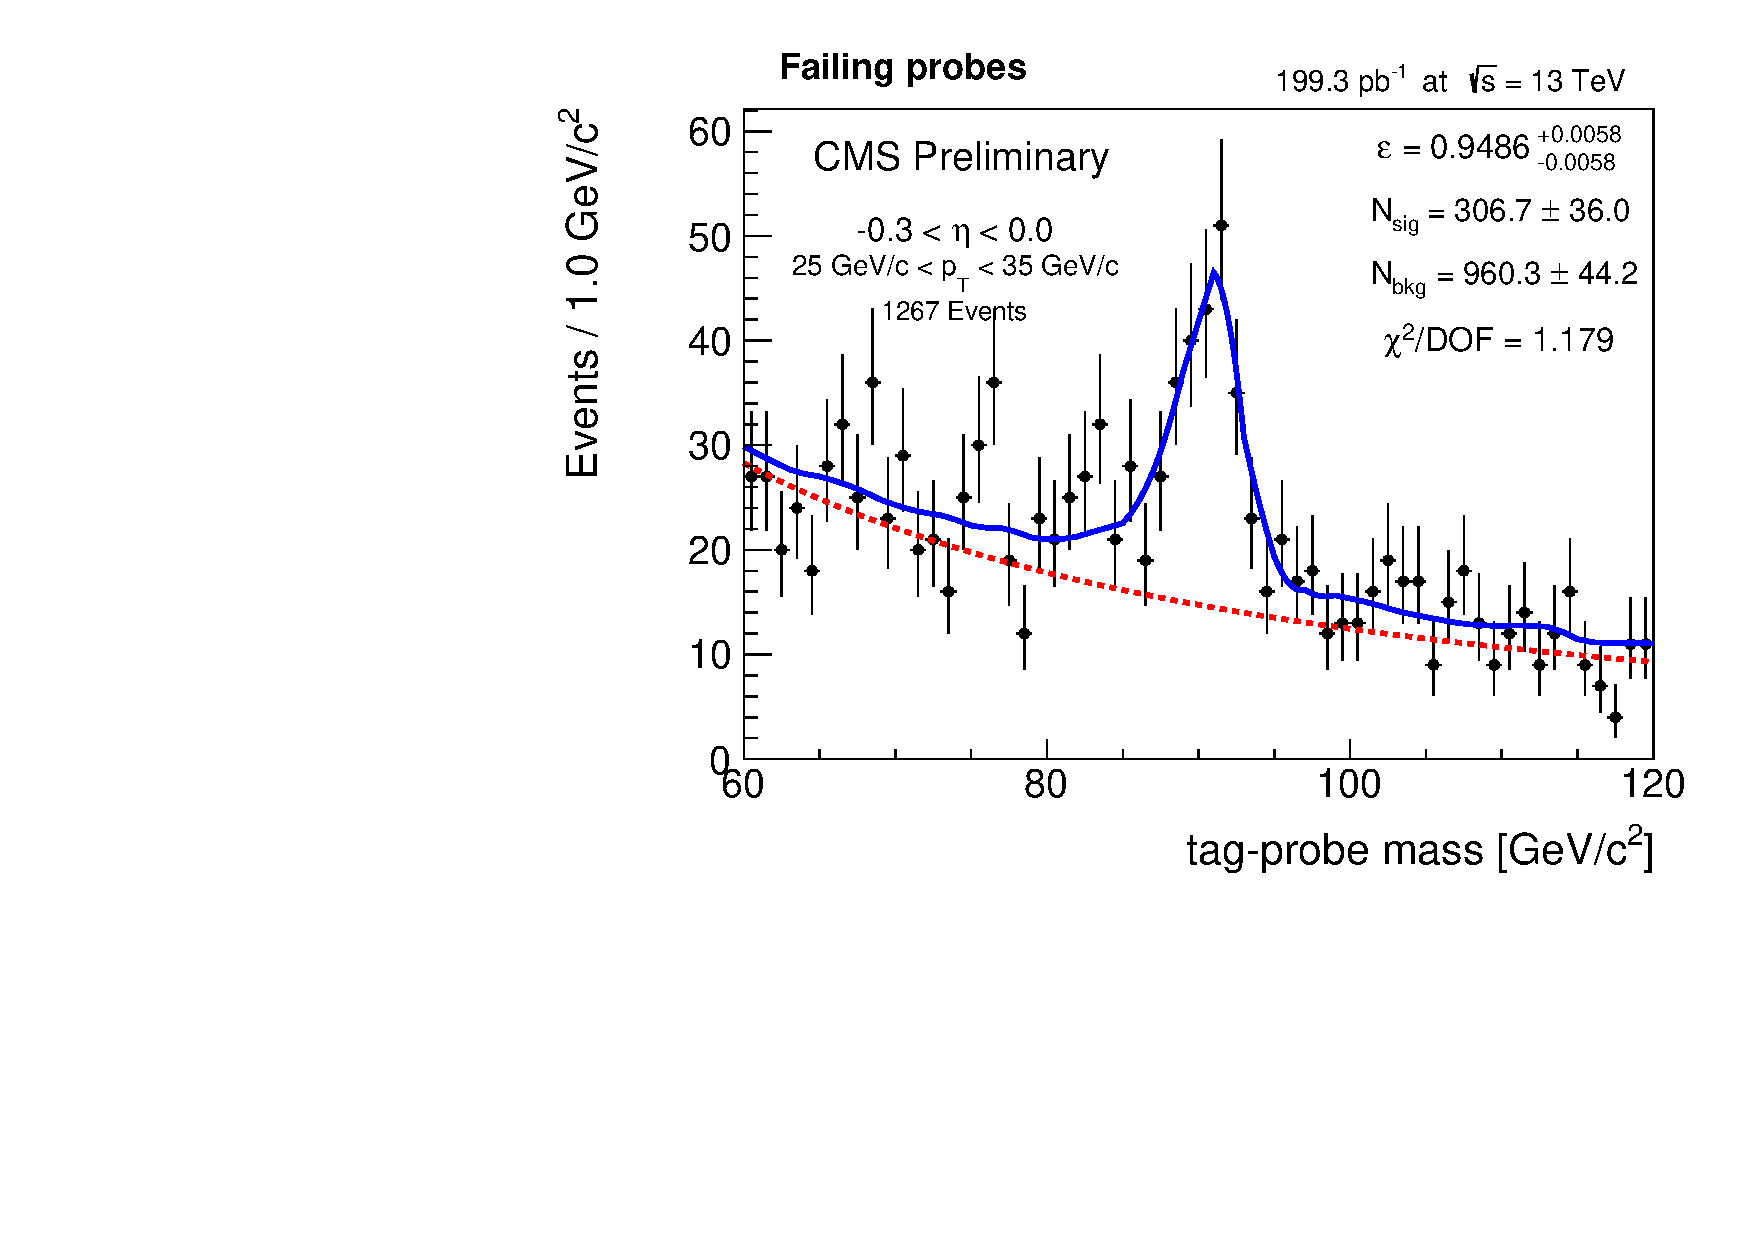
\includegraphics[width=.49\linewidth]{plots/efficiency/examples_plbkg/failetapt_5.pdf}
\caption{Examples of passing (top) and failing (bottom) probes from the same $(\pt,\eta)$ bin in the muon standalone efficiency category. The baseline efficiency value is determined using a fit with a quadratic polynomial background model (left) and uncertainties due to background model choice are evaluated using a fit with a power law background (right).}
\label{fig:eff:musta:fitexample}
\end{figure}
